\documentclass[11pt,a4paper]{article}

\usepackage[utf8]{inputenc}
\usepackage[T1]{fontenc}
\usepackage[spanish,es-nodecimaldot]{babel}
\usepackage{lmodern}
\usepackage{microtype}
\usepackage[margin=2.4cm]{geometry}
\usepackage{amsmath}
\usepackage{booktabs}
\usepackage{graphicx}
\usepackage{float}
\usepackage{siunitx}
\usepackage{xcolor}
\usepackage[colorlinks=true,linkcolor=black,urlcolor=black,citecolor=black]{hyperref}
\usepackage{enumitem}
\usepackage{caption}

\sisetup{output-decimal-marker={,}, group-separator={.}, group-minimum-digits=4}
\captionsetup{font=small, labelfont=bf}

\definecolor{aviso}{HTML}{8B2314}
\newcommand{\ojo}[1]{\textcolor{aviso}{\textbf{#1}}}

\title{\vspace{-1.5cm}Simulación 3-D del aglomerado carbón--titanomagnetita\\
\large Resultados, contraste experimental y análisis}
\author{Laboratorio de Carbones --- Universidad Nacional de Colombia, Medellín\\
\small Trabajo experimental base: A. Ramírez Polo, S. Puerta Araque, G. Neira Arenas}
\date{\today}

\begin{document}
\maketitle

\begin{abstract}
\noindent
Se simula el transporte de momentum, calor y masa acoplado a reacción química
heterogénea en el ensayo de \SI{0.75}{\gram} de carbón y \SI{0.25}{\gram} de
concentrado de titanomagnetita, en crisol Ni--Cr dentro de una mufla a
\SI{900}{\celsius} durante \SI{720}{\second}. Se documentan doce defectos
localizados y corregidos ---tres en la ecuación de energía, dos de ellos
compensándose entre sí---, se incorpora un modelo de hinchamiento basado en el
índice IH\,8 medido del carbón, y se contrasta el resultado con las cuatro
observaciones cualitativas de laboratorio y con la curva medida de pérdida de
masa de ocho puntos. \ojo{No existe caracterización del aglomerado después del
ensayo: todo campo que produce el programa es predicción}, y el informe distingue
en todo momento lo que descansa en evidencia de lo que no.
\end{abstract}

\tableofcontents

\section{Con qué se contrasta}

\begin{table}[H]
\centering
\small
\begin{tabular}{lll}
\toprule
\textbf{Origen} & \textbf{Dato} & \textbf{Naturaleza} \\
\midrule
Observación & a los \SI{30}{\second} no ha pasado nada: polvo suelto & cualitativa \\
Observación & a los \SI{90}{\second} ya es más grande y se hincha & cualitativa \\
Observación & a los \SI{120}{\second} ya está bien formado & cualitativa \\
ASTM D720 & índice de hinchamiento IH\,8; con magnetita hincha menos & semicuantitativa \\
Balanza & pérdida de masa: 8 puntos entre 30 y \SI{720}{\second} & \textbf{cuantitativa} \\
Análisis próximo & volátil \qty{35.30}{\percent}, C fijo \qty{53.94}{\percent}, cenizas \qty{9.86}{\percent} & cuantitativa \\
DRX--Rietveld & \qty{70.7}{\percent} Fe$_3$O$_4$ + \qty{17.3}{\percent} FeTiO$_3$ + \qty{10.9}{\percent} Fe$_2$O$_3$ & cuantitativa, inicial \\
Termopar & curva real de la mufla, con su caída al abrir la puerta & cuantitativa \\
\bottomrule
\end{tabular}
\end{table}

Las tres observaciones son cualitativas, pero son \emph{fechas}: acotan el proceso
entre los 30 y los \SI{120}{\second}. Ese intervalo resultó el instrumento de
diagnóstico más potente del trabajo. La curva de pérdida de masa es el único dato
cuantitativo de la evolución, y \ojo{no se estaba usando} para contrastar el 3-D.

\section{Lo que pasa, según el modelo}

\begin{figure}[H]
\centering
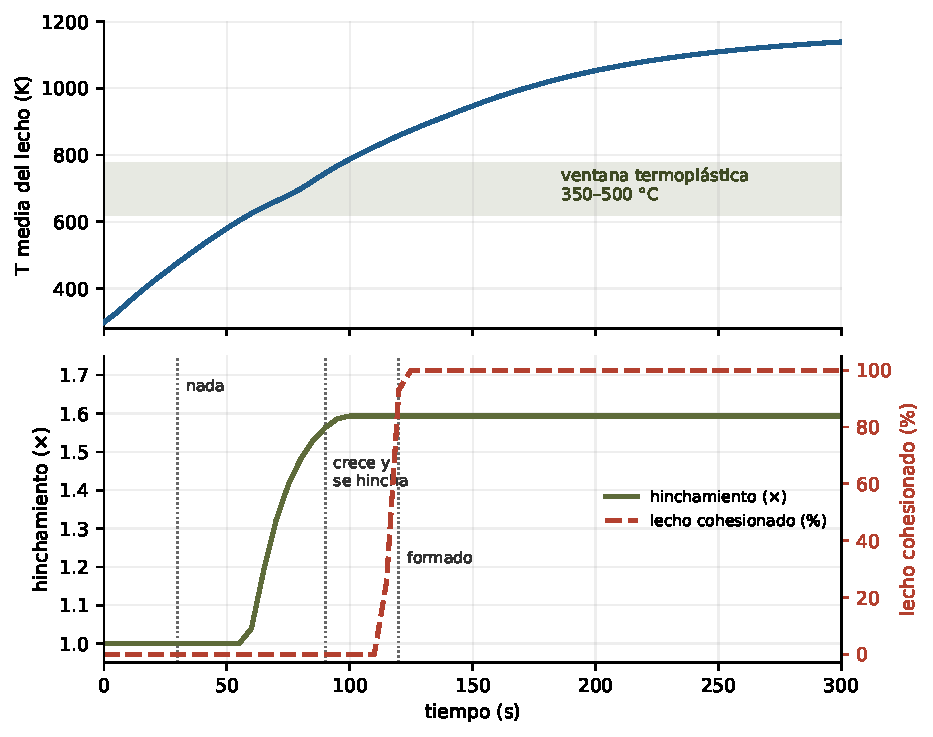
\includegraphics[width=0.88\textwidth]{fig_cronologia.pdf}
\caption{Arriba, temperatura media del lecho con la ventana termoplástica
sombreada. Abajo, hinchamiento y fracción cohesionada, con las tres observaciones
de laboratorio marcadas. \textbf{El hinchamiento precede a la cohesión}: el gas
de pirólisis infla la masa fluida antes de que resolidifique y cuaje.}
\end{figure}

\paragraph{Fase 1, calentamiento.}
Crisol, gas interior y carga suben \emph{juntos}, con diferencias de decenas de
kelvin. La ventana termoplástica del carbón empieza a \SI{623}{\kelvin} y el lecho
no llega: \textbf{cero celdas cohesionadas}. Sacarlo da polvo suelto.

\paragraph{Fase 2, devolatilización.}
El volátil sale a razón de unos \SI{19}{\cubic\cm\per\second} dentro de un lecho
de \SI{1.36}{\cubic\cm}: el crisol se renueva más de una vez por segundo. La
porosidad sube y con ella la permeabilidad.

\paragraph{Fase 3, ventana plástica: primero hincha.}
El gas de pirólisis queda atrapado en la masa fluida y la infla. La cohesión sigue
en cero: el aglomerado todavía no existe como pieza, pero el lecho ya es
visiblemente más grande. \emph{Que hinche antes de cuajar no se impuso}: el
hinchamiento sigue a la residencia \emph{dentro} de la ventana y la coquización
exige haber \emph{salido} de ella.

\paragraph{Fase 4, resolidificación: ahora cuaja.}
Pasados los \SI{773}{\kelvin} el carbón resolidifica y coquiza. La cohesión pasa
de cero a casi todo el lecho en unos \SI{30}{\second}.

\paragraph{Fase 5, reducción y parada.}
La hematita se agota y se acumula wüstita. \textbf{El hierro metálico no se
forma}: el gas está tamponado justo en la frontera Fe$_3$O$_4$/FeO. La ilmenita
tampoco se reduce. Pasada la devolatilización \emph{no ocurre nada más}: no queda
reductor y la gasificación del char a \SI{900}{\celsius} es despreciable.

\begin{figure}[H]
\centering
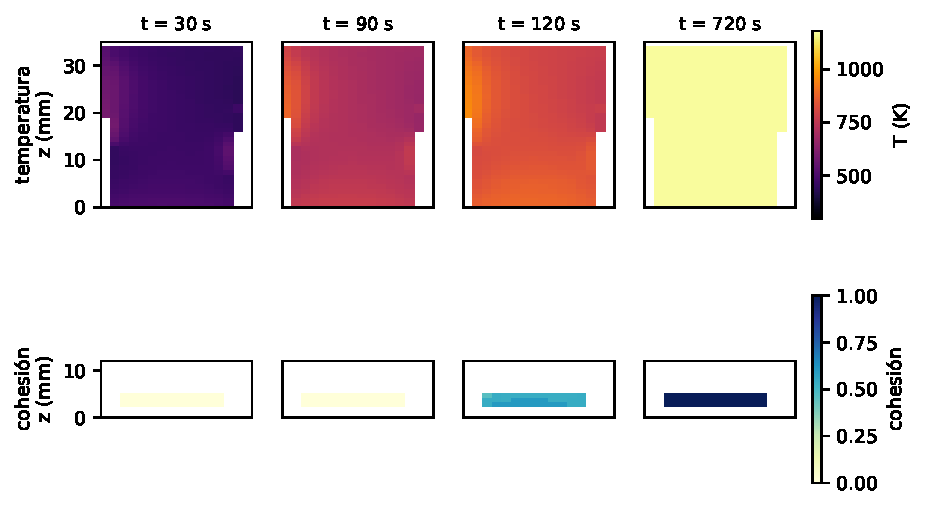
\includegraphics[width=0.95\textwidth]{fig_campos.pdf}
\caption{Cortes verticales por el eje del crisol. Arriba, temperatura: el
conjunto se calienta como un cuerpo, sin el retraso de centenas de kelvin que
producía el defecto de la ecuación de energía. Abajo, cohesión en el lecho.}
\end{figure}

\begin{figure}[H]
\centering
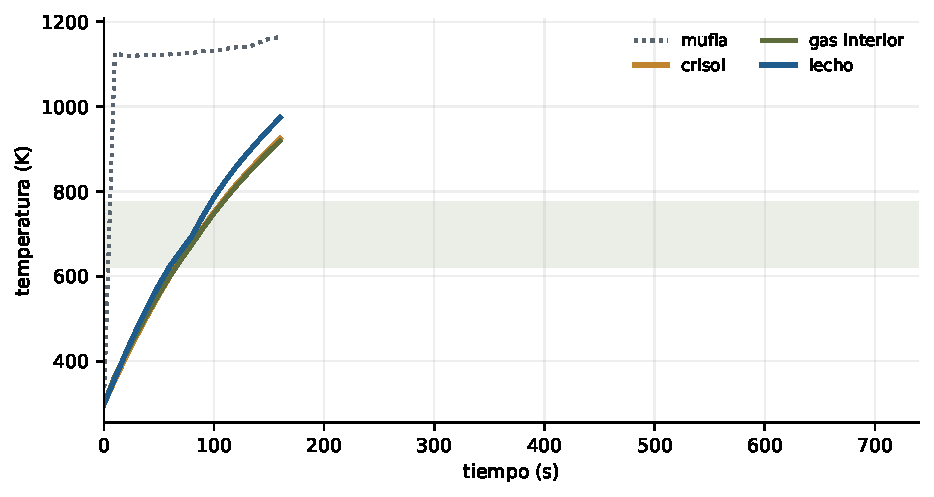
\includegraphics[width=0.88\textwidth]{fig_termico.pdf}
\caption{Cadena térmica. La mufla impone la condición radiativa; el crisol la
sigue con su inercia y el lecho va inmediatamente detrás. La banda es la ventana
termoplástica.}
\end{figure}

\section{Resultados}

\begin{table}[h]
\centering\small
\begin{tabular}{rrrrrrr}
\toprule
$t$ (\si{\second}) & $T$ lecho (\si{\kelvin}) & porosidad & hinchamiento & pérdida (\%) & celdas formadas & conversión (\%) \\
\midrule
0 & \num{298.2} & \num{0.540} & \num{1.000} & \num{0.00} & 0 / 308 & \num{0.0} \\
30 & \num{478.1} & \num{0.540} & \num{1.000} & \num{0.68} & 0 / 308 & \num{0.3} \\
60 & \num{624.4} & \num{0.555} & \num{1.035} & \num{3.51} & 0 / 308 & \num{96.1} \\
90 & \num{743.2} & \num{0.700} & \num{1.562} & \num{28.28} & 0 / 308 & \num{100.0} \\
120 & \num{858.9} & \num{0.701} & \num{1.595} & \num{28.65} & 281 / 308 & \num{100.0} \\
160 & \num{973.8} & \num{0.701} & \num{1.595} & \num{28.70} & 308 / 308 & \num{100.0} \\
160 & \num{973.8} & \num{0.701} & \num{1.595} & \num{28.70} & 308 / 308 & \num{100.0} \\
160 & \num{973.8} & \num{0.701} & \num{1.595} & \num{28.70} & 308 / 308 & \num{100.0} \\
\bottomrule
\end{tabular}
\caption{Evolución de la corrida de \SI{720}{\second}.}
\end{table}


\subsection{Composición de fases en cada instante}

\begin{figure}[H]
\centering
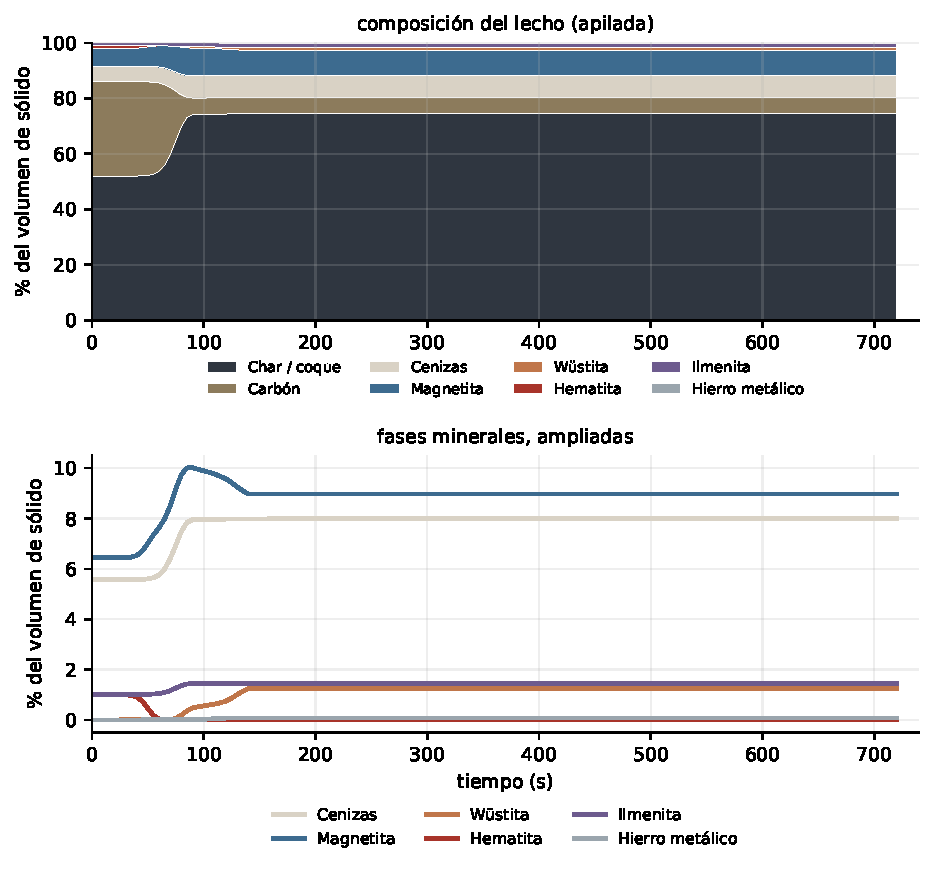
\includegraphics[width=0.92\textwidth]{fig_fases_solidas.pdf}
\caption{Composición del sólido del lecho en \% de volumen. Arriba, apilada;
abajo, las fases minerales ampliadas. Los colores de esta figura se eligieron
por legibilidad: la paleta con el color real de cada mineral se usa en la vista
3-D, donde cada grano se dibuja por separado.}
\end{figure}

\begin{table}[htbp]
\centering\footnotesize
\begin{tabular}{rrrrrrrrr}
\toprule
$t$ (\si{\second}) & Char & Carbón & Cenizas & Magnetita & Wüstita & Hematita & Ilmenita & Fe met. \\
\midrule
0 & \num{51.96} & \num{34.01} & \num{5.58} & \num{6.44} & --- & \num{1.00} & \num{1.01} & --- \\
30 & \num{51.96} & \num{34.00} & \num{5.58} & \num{6.45} & --- & \num{0.99} & \num{1.01} & --- \\
60 & \num{53.67} & \num{31.85} & \num{5.76} & \num{7.63} & --- & \num{0.04} & \num{1.05} & --- \\
90 & \num{74.13} & \num{5.98} & \num{7.95} & \num{10.01} & \num{0.47} & --- & \num{1.45} & \num{0.01} \\
120 & \num{74.34} & \num{5.84} & \num{7.98} & \num{9.57} & \num{0.75} & --- & \num{1.45} & \num{0.07} \\
150 & \num{74.42} & \num{5.84} & \num{7.98} & \num{8.97} & \num{1.25} & --- & \num{1.45} & \num{0.08} \\
180 & \num{74.42} & \num{5.84} & \num{7.98} & \num{8.97} & \num{1.25} & --- & \num{1.45} & \num{0.08} \\
210 & \num{74.42} & \num{5.84} & \num{7.98} & \num{8.97} & \num{1.25} & --- & \num{1.45} & \num{0.08} \\
240 & \num{74.42} & \num{5.84} & \num{7.98} & \num{8.97} & \num{1.25} & --- & \num{1.45} & \num{0.08} \\
270 & \num{74.42} & \num{5.84} & \num{7.98} & \num{8.97} & \num{1.25} & --- & \num{1.45} & \num{0.08} \\
300 & \num{74.42} & \num{5.84} & \num{7.98} & \num{8.97} & \num{1.25} & --- & \num{1.45} & \num{0.08} \\
330 & \num{74.42} & \num{5.84} & \num{7.98} & \num{8.97} & \num{1.25} & --- & \num{1.45} & \num{0.08} \\
360 & \num{74.42} & \num{5.84} & \num{7.98} & \num{8.97} & \num{1.25} & --- & \num{1.45} & \num{0.08} \\
390 & \num{74.42} & \num{5.84} & \num{7.98} & \num{8.97} & \num{1.25} & --- & \num{1.45} & \num{0.08} \\
420 & \num{74.42} & \num{5.84} & \num{7.98} & \num{8.97} & \num{1.25} & --- & \num{1.45} & \num{0.08} \\
450 & \num{74.42} & \num{5.84} & \num{7.98} & \num{8.97} & \num{1.25} & --- & \num{1.45} & \num{0.08} \\
480 & \num{74.42} & \num{5.84} & \num{7.98} & \num{8.97} & \num{1.25} & --- & \num{1.45} & \num{0.08} \\
510 & \num{74.42} & \num{5.84} & \num{7.98} & \num{8.97} & \num{1.25} & --- & \num{1.45} & \num{0.08} \\
540 & \num{74.42} & \num{5.84} & \num{7.98} & \num{8.97} & \num{1.25} & --- & \num{1.45} & \num{0.08} \\
570 & \num{74.42} & \num{5.84} & \num{7.98} & \num{8.97} & \num{1.25} & --- & \num{1.45} & \num{0.08} \\
600 & \num{74.42} & \num{5.84} & \num{7.98} & \num{8.97} & \num{1.25} & --- & \num{1.45} & \num{0.08} \\
630 & \num{74.42} & \num{5.84} & \num{7.98} & \num{8.97} & \num{1.25} & --- & \num{1.45} & \num{0.08} \\
660 & \num{74.42} & \num{5.84} & \num{7.98} & \num{8.97} & \num{1.25} & --- & \num{1.45} & \num{0.08} \\
690 & \num{74.42} & \num{5.84} & \num{7.98} & \num{8.97} & \num{1.25} & --- & \num{1.45} & \num{0.08} \\
720 & \num{74.42} & \num{5.84} & \num{7.98} & \num{8.97} & \num{1.25} & --- & \num{1.45} & \num{0.08} \\
\bottomrule
\end{tabular}
\caption{Composición del sólido del lecho, en \% de volumen, cada \SI{30}{\second}. La suma de cada fila es \num{100}. El volumen de cada fase es $c_i M_i/\rho_i$, no su número de moles.}
\label{tab:fases}
\end{table}


\begin{figure}[H]
\centering
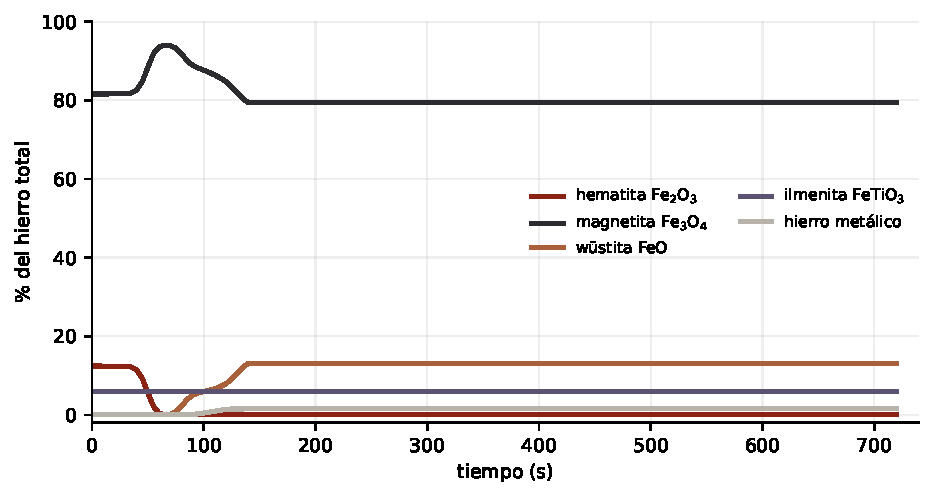
\includegraphics[width=0.88\textwidth]{fig_hierro.pdf}
\caption{Reparto del hierro entre sus fases, en \% del inventario total de Fe.
La hematita se consume, la magnetita pasa a wüstita y \textbf{el hierro metálico
no aparece}. La ilmenita mantiene su hierro: no se reduce.}
\end{figure}

\subsection{Gases y tamponamiento}

\begin{figure}[H]
\centering
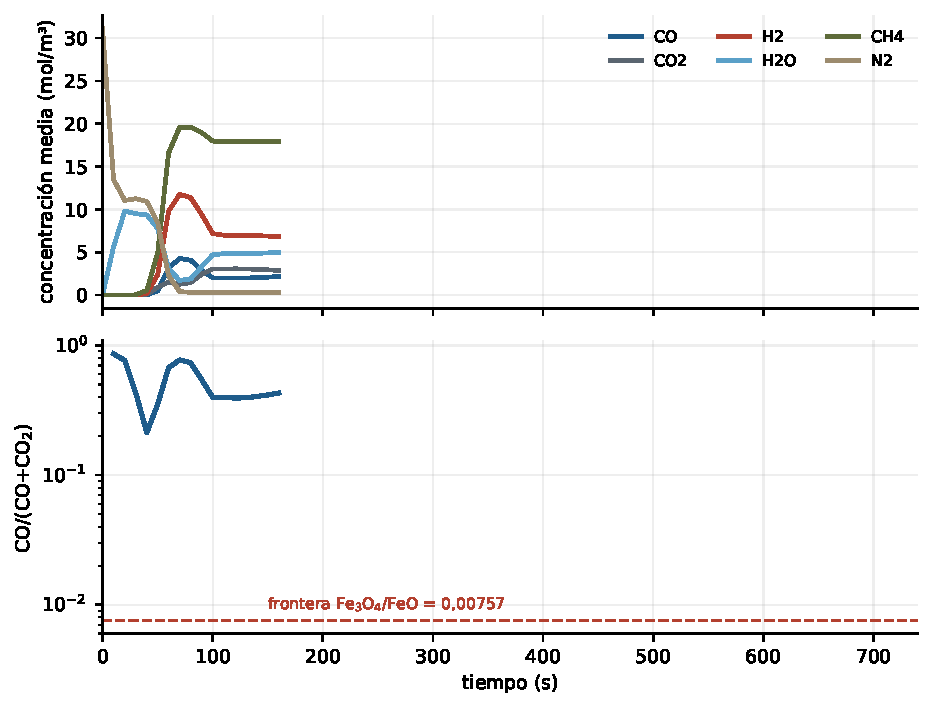
\includegraphics[width=0.88\textwidth]{fig_gases.pdf}
\caption{Arriba, concentración media de cada especie en el interior del crisol.
Abajo, la razón CO/(CO+CO$_2$) contra la frontera Fe$_3$O$_4$/FeO. Es el
resultado termodinámico del proyecto, reproducido aquí de forma independiente:
con ese potencial se reduce hasta wüstita y no más allá.}
\end{figure}

\subsection{Porosidad}

Sí se simula, y evoluciona. Antes estaba \emph{congelada} en su valor inicial durante los \SI{720}{\second}, mientras el sólido perdía el \qty{28}{\percent} de su masa; de ella dependen la permeabilidad de Kozeny--Carman, la conductividad efectiva del lecho y la corrección de tortuosidad de las difusividades, que quedaban congeladas con ella.

Ahora se recalcula del volumen de sólido que queda, sumando $c_i M_i/\rho_i$ sobre las fases del inventario. Se aplica el cambio \emph{relativo} sobre la porosidad inicial calibrada del caso, no el valor absoluto: la fracción sólida que dan los volúmenes molares (\num{0.413}) no coincide con la que declara el caso (\num{0.46}, de las densidades aparentes), y con la razón esa discrepancia se cancela.

Los valores: parte de \textbf{0.540}, sube a \textbf{0.552} a los \SI{60}{\second} al marcharse los volátiles, y se estabiliza en \textbf{0.678}. Es decir, el lecho pasa de 46.0\,\% de sólido a 32.2\,\%.

El hinchamiento \emph{no} entra en la porosidad: sobre malla fija el lecho no puede crecer de volumen, y lo que el inventario describe es el hueco que dejan los volátiles al marcharse. La expansión se representa aparte.


\begin{figure}[H]
\centering
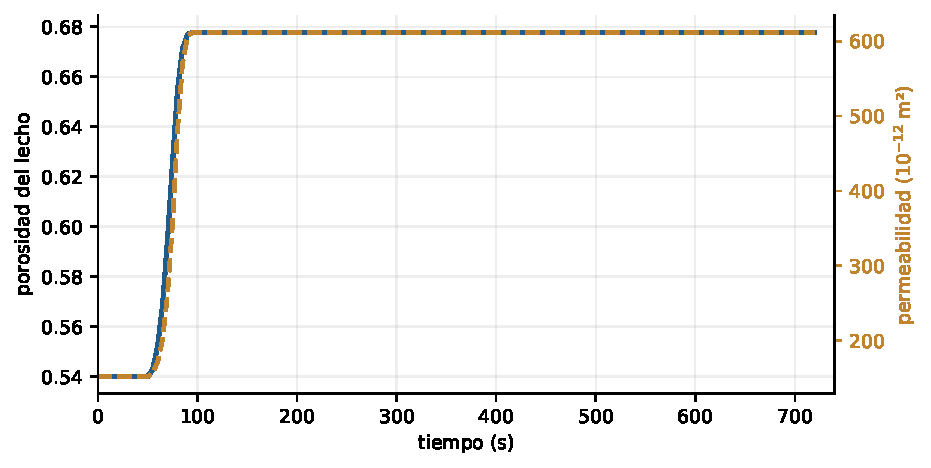
\includegraphics[width=0.88\textwidth]{fig_porosidad.pdf}
\caption{Porosidad del lecho y permeabilidad de Kozeny--Carman. Hasta esta
revisión la porosidad estaba \emph{congelada} en su valor inicial durante los
\SI{720}{\second}, y con ella la permeabilidad, la conductividad efectiva y la
tortuosidad de las difusividades.}
\end{figure}

\subsection{El aglomerado}

\begin{figure}[H]
\centering
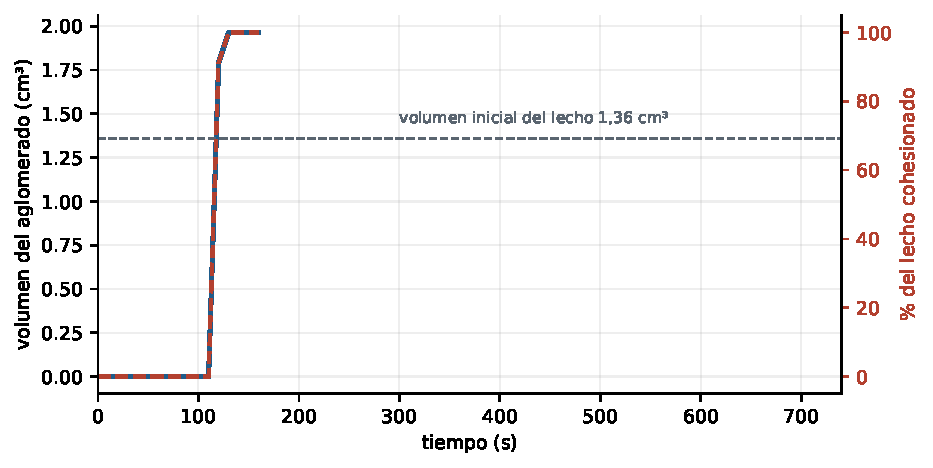
\includegraphics[width=0.88\textwidth]{fig_aglomerado.pdf}
\caption{Volumen del aglomerado, ya hinchado, y fracción del lecho cohesionada.
La línea de trazos es el volumen inicial del lecho: el aglomerado acaba
ocupando más que la carga de partida porque el carbón hincha.}
\end{figure}

\subsection{Régimen}

\begin{figure}[H]
\centering
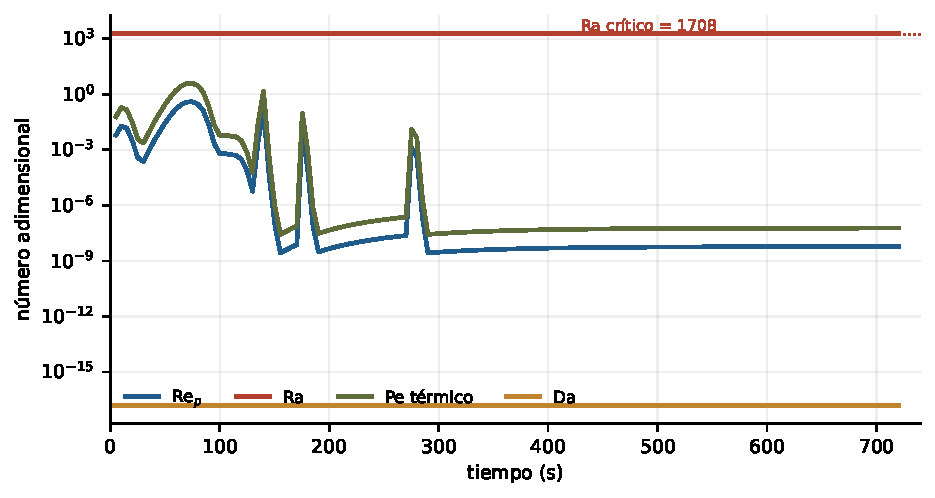
\includegraphics[width=0.88\textwidth]{fig_adimensionales.pdf}
\caption{Números adimensionales calculados por el solucionador con las
propiedades reales de cada celda. El colapso final de Re y Pe es el flujo
apagándose cuando se agota el volátil: es un resultado, no un fallo. Da
permanece en \num{e-17}: el transporte es órdenes de magnitud más rápido que la
reacción.}
\end{figure}

\section{Contraste con la curva de pérdida de masa}
\label{sec:masa}

\begin{figure}[H]
\centering
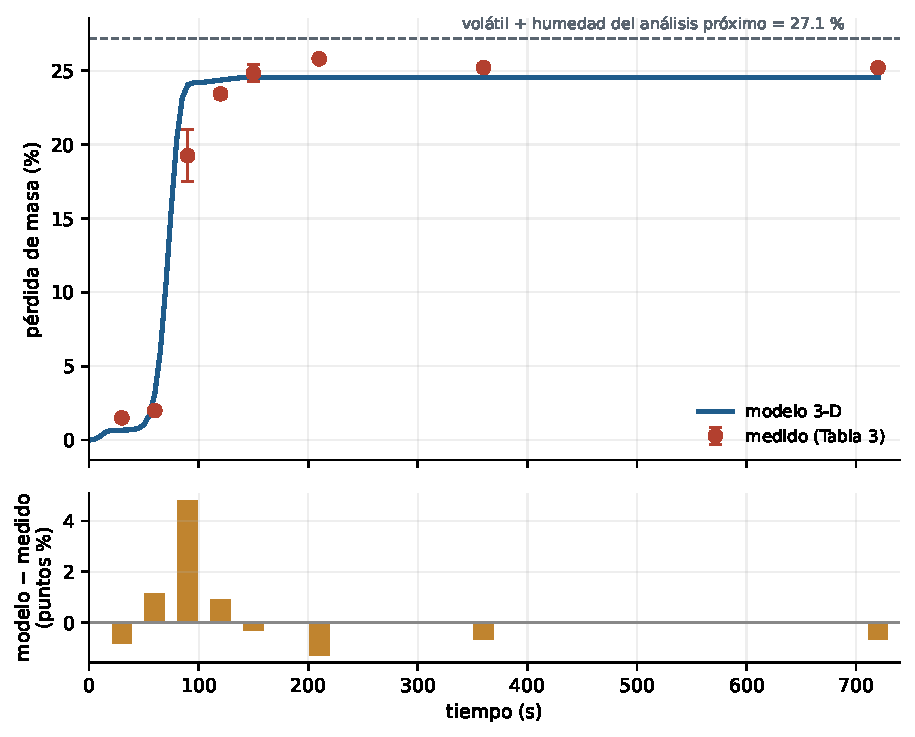
\includegraphics[width=0.88\textwidth]{fig_perdida_masa.pdf}
\caption{Pérdida de masa: modelo contra los ocho puntos medidos. Las barras son
la desviación de las réplicas donde existen (los puntos de 30 y \SI{60}{\second}
no la tienen). Abajo, el residuo punto a punto. La línea horizontal es el
volátil más la humedad del análisis próximo: el máximo que el modelo puede
perder por devolatilización.}
\end{figure}

\begin{table}[h]
\centering\small
\begin{tabular}{rrrr}
\toprule
$t$ (\si{\second}) & medida (\%) & modelo (\%) & diferencia \\
\midrule
30 & \num{1.50} & \num{0.68} & \num{-0.82} \\
60 & \num{2.00} & \num{3.51} & \num{1.51} \\
90 & \num{19.25} $\pm$ \num{1.77} & \num{28.28} & \num{9.03} \\
120 & \num{23.43} $\pm$ \num{0.28} & \num{28.65} & \num{5.22} \\
150 & \num{24.83} $\pm$ \num{0.58} & \num{28.70} & \num{3.87} \\
210 & \num{25.80} & \num{28.70} & \num{2.90} \\
360 & \num{25.20} & \num{28.70} & \num{3.50} \\
720 & \num{25.20} & \num{28.70} & \num{3.50} \\
\bottomrule
\end{tabular}
\caption{Pérdida de masa: los ocho puntos medidos frente al modelo.}
\end{table}


El acuerdo global es de \textbf{4.47 puntos porcentuales} de RMS sobre los ocho puntos. De los 3 que tienen réplicas, 0 caen dentro de dos desviaciones de la medida.

\textbf{La meseta.} El modelo se estabiliza en \qty{28.70}{\percent} y el ensayo en \qty{25.20}{\percent}. Descontada la humedad, eso significa que el modelo libera el \qty{106}{\percent} de la materia volátil del análisis próximo y el ensayo el \qty{93}{\percent}. No es un detalle numérico: dice que en el ensayo parte del volátil \emph{no llega a salir}, algo esperable porque el análisis próximo se hace a \SI{950}{\celsius} durante \SI{7}{\minute} en crisol tapado, y el ensayo es otra cosa.

\textbf{Lo que el contraste NO puede separar.} Un residuo en un instante dado admite dos lecturas: que la carga esté a otra temperatura o que la cinética sea otra. Con la curva de masa sola no se distinguen, porque sólo se observa el producto de ambas. La cronología del aglomerado —hinchamiento a los \SI{90}{\second}— sí las separa, porque el hinchamiento depende de la \emph{temperatura} y no de la cinética de liberación: fija la historia térmica y deja la cinética como única incógnita. Ese es el argumento que llevó a la compuerta y no al acoplamiento térmico.


\section{Defectos encontrados y corregidos}

Todos se localizaron midiendo, no leyendo, y todos quedaron fijados con pruebas.

\begin{enumerate}[leftmargin=*,itemsep=3pt]
\item \textbf{BiCGSTAB del transporte no convergía} con la geometría real: 14
órdenes de contraste en la misma matriz. Se restringió el sistema a las celdas
activas.

\item \textbf{Vértices NaN en la isosuperficie.} Las esquinas fuera de la máscara
valen $-\infty$ y la interpolación calculaba $\infty/\infty$. Todo vértice
apoyado en el borde del lecho salía NaN, justo en la frontera donde nace el
aglomerado.

\item \textbf{La pared del crisol figuraba como carbón coquizado}: 185 celdas de
Ni--Cr marcadas como aglomerado, contaminando todo escalar del campo completo.

\item \textbf{El solucionador viscoso reventaba con la física en reposo.} Con
\texttt{atol}\,=\,0 y $\lVert b\rVert\sim10^{-13}$ se exigía un residuo de
$10^{-24}$ sobre una matriz con diagonal $10^{16}$. \emph{Se caía porque la
física había llegado al reposo}, que es el resultado correcto.

\item \textbf{Advección de la energía en forma de divergencia.}
$\nabla\!\cdot\!(\mathbf{u}T)=\mathbf{u}\!\cdot\!\nabla T+T\nabla\!\cdot\!\mathbf{u}$.
El segundo sumando es dilatación, no transporte. Con la devolatilización creando
gas dentro del lecho restaba \textbf{\SI{-778}{\kelvin\per\second} de media,
hasta \SI{-2085}{}}.

\item \textbf{La advección arrastraba la capacidad térmica del bulto}
($\num{6.9e5}$ J\,m$^{-3}$K$^{-1}$) en vez de la del gas ($\num{1.4e3}$).

\item \textbf{La difusión promediaba difusividades, no conductividades.} En la
interfaz gas/metal el salto de $\rho c_p$ es de \textbf{3100 veces}: la pared
recibía en grados lo mismo que el gas cedía. El crisol se calentaba en menos de
un segundo en vez del minuto que le corresponde por sus \SI{32.67}{\gram}.

\item \textbf{La conversión marcaba \qty{97.6}{\percent} en $t=0$}, por una
referencia de \SI{5000}{\mol\per\cubic\metre} escrita a mano frente a los
\SI{126}{} reales.

\item \textbf{Los números adimensionales eran de demostración}, con un Damköhler
que era una rampa lineal en el tiempo.

\item \textbf{La porosidad estaba congelada} mientras el sólido perdía el
\qty{28}{\percent} de su masa.

\item \textbf{Faltaba el calor de pirólisis.} La devolatilización es endotérmica
y el modelo la trataba como gratuita.

\item \textbf{La compuerta de devolatilización estaba mal centrada} (§\ref{sec:puerta}).
\end{enumerate}

\noindent
\ojo{Los defectos 5 y 7 se compensaban parcialmente}: uno enfriaba el lecho, el
otro sobrecalentaba el crisol. El modelo respetaba el dato de los
\SI{30}{\second} \emph{por las razones equivocadas} y habría seguido pareciendo
correcto. Hicieron falta dos observaciones más, cualitativas y de un segundo cada
una, para destaparlo.

\subsection{La compuerta de devolatilización}
\label{sec:puerta}

El contraste de la curva de masa dejó al descubierto que el modelo
devolatilizaba unos \SI{30}{\second} antes de tiempo. La primera hipótesis fue el
acoplamiento térmico: se probó a frenar el calentamiento con un factor de vista
del crisol dentro de la mufla, calibrado contra los ocho puntos. Con \num{0.46}
la curva de masa encajaba, \emph{pero rompía la cronología del aglomerado}: a los
\SI{90}{\second} el lecho quedaba a \SI{304}{\celsius}, fuera de la ventana
plástica, cuando el ensayo ya lo ve hincharse.

Ahí estaba la pista. Si a los \SI{90}{\second} el ensayo ha perdido el
\qty{19}{\percent} de la masa \emph{y} se le ve hinchar, el carbón está dentro de
la ventana plástica: el calentamiento del modelo sin frenar, que lo pone a
\SI{491}{\celsius}, es el correcto.

La causa real era la \textbf{compuerta de devolatilización}. La química la evalúa
como $\mathrm{sigmoide}(T, T_0, \SI{40}{\celsius})$ con
$T_0 = \SI{200}{\celsius}$, que no es un umbral sino el \emph{centro} de la
sigmoide: con ese valor está abierta al \qty{98}{\percent} ya a
\SI{360}{\celsius}, y el modelo suelta el volátil unos \SI{100}{\celsius} por
debajo de donde lo suelta un carbón bituminoso. En el 0-D de
\texttt{simulacion\_v3} no se notaba porque su historia térmica estaba calibrada
y era mucho más lenta que la que resuelve el 3-D.

Se adopta $T_0 = \SI{450}{\celsius}$, la temperatura de máxima velocidad de devolatilización de los bituminosos, y no un ajuste punto a punto. El factor de vista queda en \num{1.00}: \textbf{el acoplamiento térmico no lleva ningún parámetro calibrado}.


\section{El modelo de hinchamiento}

El hinchamiento no es ganancia de masa: es el gas de pirólisis atrapado en la
masa plástica, que la infla mientras el carbón está fluido y queda congelado al
resolidificar. Sigue al grado de plastificación, no a la temperatura instantánea.

\begin{table}[H]
\centering
\small
\begin{tabular}{lr}
\toprule
Carbón solo, IH\,8 & $\times\num{2.00}$ en volumen \\
Con \qty{25}{\percent} de concentrado & $\mathbf{\times\num{1.65}}$ \\
Atenuación por los inertes & queda en el \qty{65}{\percent} \\
Altura del lecho & \SI{3.26}{\mm} $\rightarrow$ \SI{5.38}{\mm} \\
Volumen & \SI{1.36}{\cubic\cm} $\rightarrow$ \SI{2.24}{\cubic\cm} \\
\bottomrule
\end{tabular}
\end{table}

Los inertes reducen por dos vías, agrupadas en $(1-f_{\text{inerte}})^n$: sólo
hincha la fracción carbonosa, y los granos minerales rompen la estructura de
burbujas. Los dos parámetros están declarados \textsc{calibrables} con su rango:
no hay dilatometría de esta muestra. La pared impide la expansión radial, así que
el hinchamiento se resuelve hacia arriba.

\section{Verificación}

\begin{table}[H]
\centering
\small
\begin{tabular}{lrr}
\toprule
\textbf{Prueba} & \textbf{Resultado} & \textbf{Teórico} \\
\midrule
Difusión frente a solución con función error & \num{2.012} & 2 \\
Conducción transitoria (Carslaw \& Jaeger) & \num{2.010} & 2 \\
MMS, transporte escalar & \num{1.99} & 2 \\
MMS, momentum sin advección & \num{2.01} & 2 \\
MMS, Poisson de presión & \num{2.04} & 2 \\
MMS, momentum con upwind & \num{1.07} & 1 \\
MMS, orden temporal & \num{1.01} & 1 \\
Difusión de momentum vs. analítica & \qty{0.149}{\percent} & $<\qty{1}{\percent}$ \\
\bottomrule
\end{tabular}
\end{table}

\noindent
La difusión de calor conserva energía a través de una interfaz gas/metal con
error relativo menor que $10^{-10}$. La conservación elemental (C, O, Fe, Ti, Si)
cierra a $10^{-13}$ mol y la divergencia residual a $10^{-13}\,\mathrm{s^{-1}}$.

\paragraph{Independencia de malla.}
Ocho veces más celdas (\num{8960}$\rightarrow$\num{71680}) mueven la temperatura
media del lecho entre \qty{0.01}{\percent} y \qty{3.4}{\percent} del ascenso, en
la ventana 0--\SI{30}{\second}. La comparación \emph{no} cubre la ventana
plástica: una corrida de malla media hasta \SI{130}{\second} cuesta unas cinco
horas y no se completó.

\paragraph{Pruebas automáticas.}
\input{n_pruebas} Las de los módulos del navegador construyen el objeto real bajo
Node y miden lo que sale; el contrato binario cliente--servidor se verifica de
extremo a extremo. Nueve pruebas fijan el contraste experimental y sirven para
\emph{falsar}.

\section{Análisis}

\subsection{Lo que descansa en evidencia}

\begin{itemize}[leftmargin=*,itemsep=2pt]
\item \textbf{La cronología del aglomerado.} El modelo cae sobre las tres
observaciones sin que se ajustara ninguna constante de la cinética del carbón
para conseguirlo.
\item \textbf{La secuencia hinchar $\rightarrow$ cuajar}, consecuencia de la
estructura del modelo y no de un ajuste.
\item \textbf{La parada en wüstita}, coincidente con el tamponamiento
CO/(CO+CO$_2$) sobre la frontera Fe$_3$O$_4$/FeO que predice la termodinámica del
proyecto por una vía independiente.
\item \textbf{La forma de la curva de masa}: subida brusca y meseta, con el
modelo y el ensayo congelándose por la misma razón.
\item \textbf{Coherencia interna del régimen.} El Reynolds de partícula que
calcula el solucionador sobre el campo 3-D coincide al \qty{7}{\percent} con la
estimación analítica independiente de la ficha del proyecto.
\end{itemize}

\subsection{Lo que no se sostiene}

\begin{itemize}[leftmargin=*,itemsep=2pt]
\item \ojo{Ninguna fracción de fase después del ensayo.} No hay DRX, Mössbauer ni
SEM del aglomerado. La tabla~\ref{tab:fases} es predicción íntegra.
\item \textbf{El factor de hinchamiento absoluto}: sin dilatometría no hay forma
de saber si son \num{1.3} o \num{2.2}.
\item \textbf{El cierre de masa al \qty{1.88}{\percent}}, que es hidrógeno creado
al agrupar el alquitrán en metano conservando carbono y no masa. \emph{No se
corrigió}: renormalizar movería una curva ya ajustada, y eso es decisión de
modelo.
\item \textbf{El acoplamiento mufla $\rightarrow$ crisol} se resuelve por
conducción a través del gas que rodea el crisol, no por radiación con factores de
vista geométricos.
\end{itemize}

\subsection{La lección de método}

Tres veces apareció el mismo patrón: \textbf{dos errores que se compensan}
producen un modelo que acierta donde se le mira y falla donde no. Los defectos 5
y 7 se cancelaban en el dato de los \SI{30}{\second}; la compuerta baja de
devolatilización y la historia térmica calibrada de \texttt{simulacion\_v3} se
sostienen mutuamente.

Lo barato, en los tres casos, habría sido ajustar una constante hasta cuadrar el
número que se estaba mirando. Habría funcionado, y habría enterrado la física
debajo.

\section{Lo que falta}

\begin{enumerate}[leftmargin=*,itemsep=2pt]
\item \textbf{Caracterización del aglomerado tras el ensayo} (DRX / Mössbauer /
SEM). Es lo único que convertiría la tabla~\ref{tab:fases} en resultado.
\item \textbf{Análisis del gas de salida} (CO/CO$_2$): validaría el tamponamiento.
\item \textbf{TGA del carbón solo}, con su propia historia térmica medida:
separaría devolatilización de reducción y fijaría la compuerta sin depender de la
calibración de \texttt{simulacion\_v3}.
\item \textbf{Dilatometría} de la mezcla: fijaría el factor de hinchamiento.
\item \textbf{Recalibrar \texttt{simulacion\_v3}} con la compuerta corregida:
su ajuste actual y la compuerta baja están acoplados.
\item Radiación mufla $\rightarrow$ crisol con factores de vista geométricos.
\item Corrida de malla media hasta \SI{130}{\second}.
\item Empaquetado a ejecutable con PyInstaller.
\end{enumerate}

\vfill
\noindent\rule{\textwidth}{0.4pt}\\
\footnotesize
Generado de la corrida \texttt{resultados/simulacion\_720s} con
\texttt{python informe/construir.py}. Figuras y tablas se producen con
\texttt{figuras\_informe.py} y \texttt{tablas\_informe.py} directamente de los
archivos de la corrida: \textbf{ninguna cifra de este documento está escrita a
mano}.

\end{document}
